\documentclass{article}
\usepackage[utf8]{inputenc}
\usepackage{amsmath}
\usepackage{enumerate}
\usepackage{graphicx}
\usepackage{tikz}
\usetikzlibrary{bayesnet}
\usepackage{microtype}
\usepackage{float}

\usepackage[
backend=biber,
style=numeric,
citestyle=numeric
]{biblatex}
 
\addbibresource{tm-bib.bib}

\title{Topic Modeling and Clustering}
\author{Melody Jiang}
\date{May 2019}

\begin{document}

\maketitle

\tableofcontents



\section{Introduction}

Three main tasks in textmining are clustering, classification, and information extraction \cite{allahyari2017brief}. Topic modeling can be applied to all of these tasks \cite{lu2011investigating}. We would like to focus on the most commonly used topic model, Latent Dirichlet Allocation (LDA), and its performance in the documeng clustering task. Lu et al. investigated LDA's task performance in document clustering and found LDA's performance is quite sensitive to the setting of its hyper-parameter and parameter \cite{lu2011investigating}. In terms of robustness, Wang et al. proposed a model-based approach to make LDA more robust by using localization and empirical Bayes \cite{wang2018general}.

In this section, we review types of clustering methods in text clustering, Latent Dirichlet Allocation (LDA), and evaluation metrics for clustering and LDA. In the following sections, we would present simulation experiments. We first verified that performance of LDA is sensitive to settings of hyperparameter $\alpha$. We then attempted incorporating perturbation in posterior samples and tested perturbation on Dirichlet-Multinomial. At last, we discuss the current idea of using proper scoring rules and cross validation to tune the hyperparameter $\alpha$.


\subsection{Types of document clustering}

\textbf{Hard Clustering versus Soft Clustering.} Hard clustering computes a hard assignment of each document to a specific cluster. That is, each document is a member of exactly one cluster. In soft clustering, a document's assignment is a distribution over all clusters \cite{manning2008iir}. Hard clustering can be seen as a special case of soft clustering.

\textbf{Model-based Clustering versus Distance-based Clustering.} Model-based clustering assumes that the data were generated by a model and tries to recover the original model from the data. A commonly used criterion for estimating the model parameters is maximum likelihood, and the expectation-maximization(EM) algorithm is commonly used for such computation \cite{manning2008iir}.

Distance-based clustering algorithms use a similarity function to measure the closeness between text objects \cite{aggarwal2012mining}. Two most widely used distanced-based clustering algorithms are k-medoid clustering algorithm and k-means clustering algorithms \cite{aggarwal2012mining,manning2008iir}.

\textbf{Flat Clustering versus Hiearchical Clustering} Flat clustering creates a flat set of cluster without any explicit structure that would relate clusters to each other while Hierarchical clustering creates a hierarchy of clusters \cite{manning2008iir}.





\subsection{Latent Dirichlet Allocation (LDA)}

In this section, we reproduce the LDA model described in \cite{wang2018general} and \cite{blei2009topic}.

Let:

\begin{itemize}
  \item $K$ be a specified number of topics,
  \item $D$ the number of documents,
  \item $N_d$ the number of words in a document,
  \item $V$  the size of the vocabulary,
  \item $\boldsymbol{\alpha}$ a positive K-vector,
  \item $\eta$ a scalar. 
  \item $Dir_K(\boldsymbol{\alpha})$ a K-dimensional Dirichlet distribution with vector parameter $\boldsymbol{\alpha}$,
  \item $Dir_V(\eta)$ a V-Dimensional symmetric Dirichlet distribution with scalar parameter $\eta$.
\end{itemize}

A \textit{symmetric Dirichlet} is a Dirichlet distribution where each component of the parameter is equal to the same value.

We define each topic $\boldsymbol{\beta}_k$ to be a distribution over a fixed vocabulary and we fix the number of topics $K$. LDA assumes that a collection of documents comes from the following process:

\begin{enumerate}
  \item Draw each topic $\boldsymbol{\beta}_k \sim Dir_V(\eta)$ for k = 1, 2, ..., K.
  \item For each document $d$ ($d = 1, ..., D$),
  \begin{enumerate}
    \item Draw a vector of topic proportions $\boldsymbol{\theta}_d \sim Dir_K(\boldsymbol{\alpha})$
    \item For each word $w_n$ ($n = 1, ..., N_d$) in document $d$,
    \begin{enumerate}
      \item Draw topic assignment $z_{dn} \sim Mult(\boldsymbol{\theta}_d)$, where $z_{dn} \in \{1, ..., K\}$.
      \item Draw word $w_{dn} \sim Mult(\boldsymbol{\beta}_{z_{dn}})$, where $w_{dn} \in \{1, ..., V\}$.
    \end{enumerate}
  \end{enumerate}
\end{enumerate}

See Figure \ref{fig:gaphical_model_lda} for a directed graphical model of LDA.

\begin{figure}
  \centering
  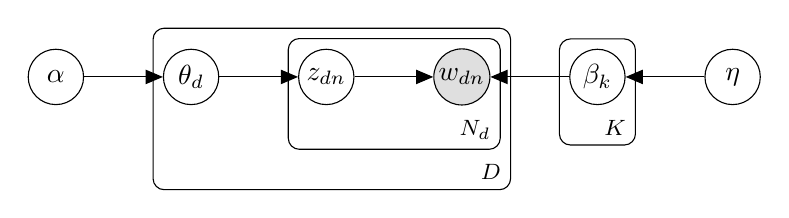
\begin{tikzpicture}

    % Nodes
    \node[obs] (w) {$w_{dn}$}; %word
    \node[latent, right=of w] (beta) {$\beta_k$}; %topic
    \node[latent, right=of beta] (eta) {$\eta$}; % eta
    \node[latent, left=of w] (z) {$z_{dn}$}; % topic assignment of word
    \node[latent, left=of z] (theta) {$\theta_d$}; % topic proportion of a document
    \node[latent, left=of theta] (alpha) {$\alpha$}; % hyperparameter alpha
  
    % Edge
    \edge {beta} {w}; % arrow pointing from topic to word
    \edge {eta} {beta}; % arrow pointing fromm eta to beta
    \edge {z} {w} % arrow pointing from topic assignment to word
    \edge {theta} {z} % arrow pointing from topic porportion of a document to topic assignment of a word
    \edge {alpha} {theta} % arrow pointing from hyperparameter alpha to topic proportion of a document
  
    % Plates
    \plate {wordPlate} {(w)(z)} {$N_d$};
    \plate {documentPlate} {(wordPlate)(theta)} {$D$};
    \plate {} {(beta)} {$K$};
  
  \end{tikzpicture}
  \caption{The directed graphical model of LDA. Adapted from \cite{blei2012probablistic} and \cite{blei2009topic}. Nodes denote random variables; edges denote dependence between random variables. Shaded nodes denote observed random variables; unshaded nodes denote hidden random variables. The rectangular boxes are ``plate notation", which denote replication.}
  \label{fig:gaphical_model_lda}
\end{figure}


\subsubsection{Likelihood functions of LDA}

\begin{align}
  p_d(w | \{\boldsymbol{\beta}_k\}_{1:K}, \boldsymbol{\theta}_d) = \sum_{k = 1}^K \theta_{dk} p(w | \boldsymbol{\beta}_k)
\end{align}

\begin{align}
  & p(d | \boldsymbol{\alpha}, \{\boldsymbol{\beta}_k\}_{1:K}) \\
  & = \int \left\{ \prod_{w \in V} \left[ \sum_{k = 1}^K \theta_{dk} p(w | \boldsymbol{\beta}_k) \right]^{c(w,d)} \right\} p(\boldsymbol{\theta}_d | \boldsymbol{\alpha}) d\boldsymbol{\theta}_d
\end{align}


\subsection{Evaluation}

Evaluation of clustering includes using internal criterion and external criterion for evaluation. Most objective functions in clustering formalize the goal of attaining high intracluster similarity and low inter-cluster similarity. That is, in the context of text clustering, documents within a cluster are similar and documents from different clusters are dissimilar. This is an internal criterion for the quality of a clustering. However, good scores on an internal criterion do not necessarily mean effectiveness in applications \cite{manning2008iir}.

To ensure effectiveness in applications, one can compute an external criterion that evaluates how well clustering matches an evaluation benchmark or gold standard \cite{manning2008iir}. Commonly used external criteria include purity, normalized mutual information, Rand index, and F measure \cite{manning2008iir}. Purity is simple and transparent. Normalized mutual information has the advantage of being able to be information-theoretically interpreted. The Rand index penalizes both false-positive and false-negative decisions during clustering. The F meassure not only penalizes false-negative and falose-positive decisions, but also supports differential weighting of these two types of errors \cite{manning2008iir}. The gold standard is ideally produced by human judges with a good level of inter-judge agreement. Historically, the Reuters-21578 collection was the main benchmark for text classification evaluation and is commonly used in evaluation of text clustering \cite{manning2008iir}.

Outside of the contexts in applications, topic models on their own are most commonly evaluted by using perplexity \cite{Griffiths5228}. As described in \cite{blei2003latent}, the perplexity is monotonically decrasing in the likelihood of the testing data, and perplexity is algebratically equivalent to the inverse of the geometric mean per-word likelihood. A lower perplexity score indicates better generalization performance of the model. For a testing dataset that consists of $M$ documents, the perplexity is:

$$
\text { perplexity }\left(D_{\text { test }}\right)=\exp \left\{-\frac{\sum_{d=1}^{M} \log p\left(\mathbf{w}_{d}\right)}{\sum_{d=1}^{M} N_{d}}\right\}
$$.






\section{Experiment: How $\alpha$ affects performance of LDA}

We performed experiments similar to those in \cite{lu2011investigating}. We investigated how the hyperparameter $\alpha$ and the total number of topics $K$ affect LDA's performance in document clustering.

We used the Reuters-21578 R8 \footnote{https://www.cs.umb.edu/~smimarog/textmining/datasets/} dataset. Reuters-21578 R8 is a pre-processed subset of Reuters-21578, \footnote{http://www.daviddlewis.com/resources/testcollections/reuters21578/} a very widely used dataset in textmining research. Training data and testing data are provided in two separate files.

All analyses were done in R.

\subsection{Preprocessing}

First, we subset training data to 3 document classes (topics) for computational expense. We did the same for testing data.

Similar to what was done in \cite{lu2011investigating}, we studied LDA in the standard clustering setting, where each document belongs to exactly one cluster. Hence, we removed documents appearing in two or more categories. Now we end up with 679 documents for training data and 279 documents for testing data.

As we have mentioned, Reuters-21578 R8 is a pre-processed subset of Reuters-21578. Preprocessing that has already been done for us are:

\begin{enumerate}
  \item Substituteing TAB, NEWLINE and RETURN characters by SPACE;
  \item Keeping only letters (i.e., turn punctuation, numbers, etc. into SPACES);
  \item Turning all letters to lowercase.
  \item Substituting multiple SPACES by a single SPACE.
  \item The title/subject of each document is simply added in the beginning of the document's text.
\end{enumerate}

Preprocessing steps performed by us are stopword removal and stemming. Tokenization was automatically performed when we create document-term matrices. After preprocessing, there were 5291 terms in the vocabulary.


\subsection{Evaluation Metric}

We used perplexity of testing set as our evaluation metric, since the documents in the corpora are treated as if they were unlabeled. Perplexity is commonly used in topic modeling literature \cite{blei2003latent,blei2007correlated}. Other different evaluation metrics worth considering for future experiments include per-word predictive log likelihood used in \cite{wang2018general} and normalized mutual information used in \cite{lu2011investigating}.


\subsection{Results}

First, using Gibbs sampling as estimation method, we calculate perplexity for $K = 2, 3, ..., 10$. $\alpha$ was estimated by the algorithm. See Figure \ref{fig:gibbs_diff_k_10} for result.

\begin{figure}[h]
  \centering
  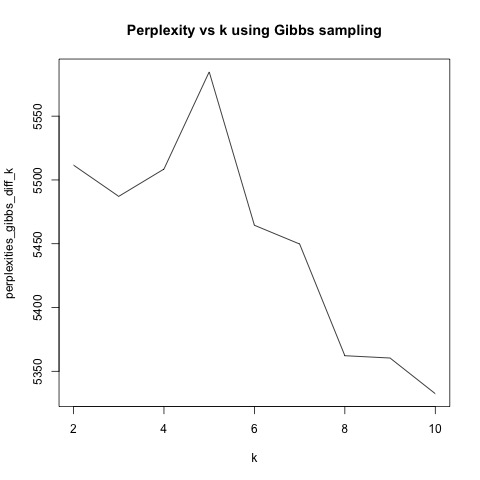
\includegraphics[width=0.5\linewidth]{images/gibbs_diff_k.jpg}
  \caption{Perplexity versus number of topics, Gibbs sampling}
  \label{fig:gibbs_diff_k_10}
\end{figure}

Then, using variational expectation-maximization (VEM) instead of Gibbs sampling as estimation method, we again calculated perplexity for $K = 2, 3, ..., 10$. $\alpha$ was still estimated by the algorithm. See Figure \ref{fig:vem_diff_k_10} for result.

\begin{figure}[h]
  \centering
  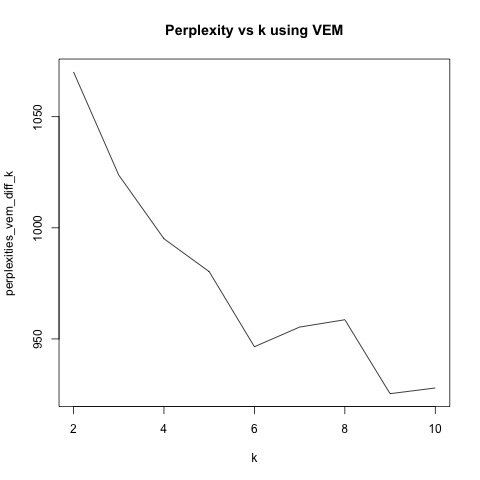
\includegraphics[width=0.5\linewidth]{images/vem_diff_k.jpg}
  \caption{Perplexity versus number of topics, VEM}
  \label{fig:vem_diff_k_10}
\end{figure}

At last, we used VEM as estimation method, fixed the number of topics $K$ to be 3, and calculated perplexity for different values of $\alpha$. Recall that we subsetted both training and testing data to be having 3 topics during preprocessing, so 3 was the actual number of topics for both training and testing data. See Figure \ref{fig:vem_diff_alpha} for results. Lu et al. investigated clustering-task peformance of LDA under $\alpha = 0.01, 0.1, 1, 5, 10, 25$ \cite{lu2011investigating} using normalized mutual information. We emulated them and examined perplexity under these settings. However, since the Dirichlet prior should be sensitive to small changes in its parameters in high-dimensional setting, we examine $30$ unevenly spaced values between $0.001$ and $1$ as well.

\begin{figure}[H]
  \centering
  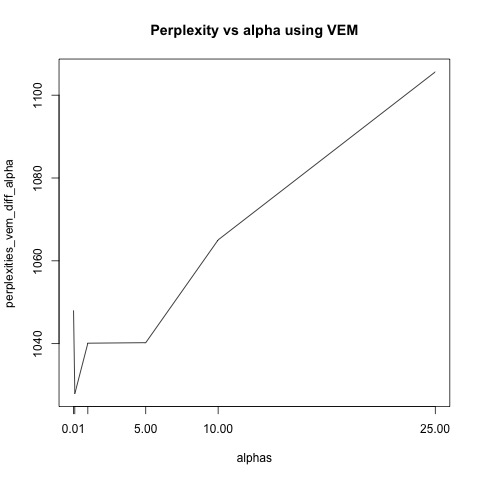
\includegraphics[width=0.5\linewidth]{images/vem_diff_alpha.jpg}
  \caption{Perplexity versus $\alpha$, VEM}
  \label{fig:vem_diff_alpha}
\end{figure}

\begin{figure}[H]
  \centering
  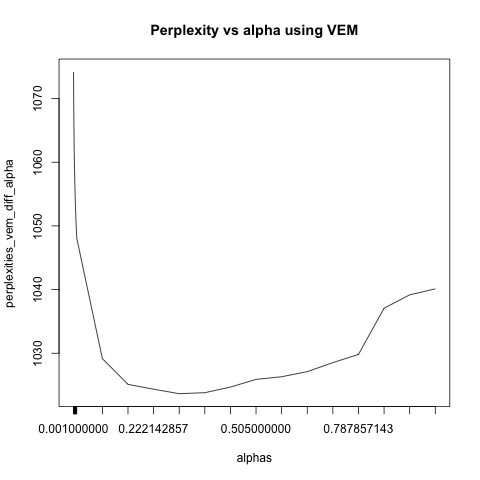
\includegraphics[width=0.5\linewidth]{images/vem_diff_alpha_small.jpg}
  \caption{Perplexity versus $\alpha$, VEM}
  \label{fig:vem_diff_alpha_small}
\end{figure}


\subsection{Discussion}

LDA is sensitive to the number of topics $K$ and the hyperparameter $\alpha$.

From Figure \ref{fig:gibbs_diff_k_10} and Figure \ref{fig:vem_diff_k_10}, we observe that the model tends to perform better on test data with a larger number of topics, despite that the actual number of topics is 3. This contradicts our expectation that large number of topics would cause the model to overfit and perform poorly on test data.

Figure \ref{fig:vem_diff_alpha} shows that LDA performs best when $\alpha$ is 0.1, and the performance worsen as $\alpha$ increases. This results agrees with the result in \cite{lu2011investigating}. The reason we obtain such result might be, as \cite{lu2011investigating} explained, while a larger value of $\alpha$ leads to more smoothed topics, $\alpha$ smaller than $1$ would cause the modes of the Dirichlet distribution to concentrate at corners of the simplex, thus favoring more sparse topics. Since we limited each document in our data to be in only one cluster, we would expect LDA to assgin a skewed topic distribution to a document. Therefore, a smaller $\alpha$ should result in better performance. However, as shown in Figure \ref{fig:vem_diff_alpha_small}, we also observe that $\alpha$ too close to $0$ ($\alpha \in [0.001, 0.1]$) results in significant decline of performance. This indicates sensitivity of LDA to settings of $\alpha$. 

For future improvements on this experiment, we would add measures other than perplexity to evaluate task performance of LDA on clustering. We could also investigate the relationship between perplexity and settings of parameters and propose better evaluation metrics.


\section{Experiment: Perturbation}

To address the issue that Dirichlet is sensitive to small changes in its parameters in high dimensional settings, our first idea was to add perturbation to posterior samples. To examine what happens when we add perturbation, we started with the simple model of Dirichlet multinomial in a high dimensional setting.

\subsection{Dirichlet Multinomial}

The multinomial sampling distribution is used to describe data for which each observation is one of k possible outcomes.

If $y$ is the vector of counts of the number of observations of each outcome, then $$p(y|\theta) \propto \prod_{j = 1}^k \theta_j^{y_j}$$, where the sum of the probabilities, $\sum_{j = 1}^k \theta_j = 1$.

The distirbution is typically thought of as implicitly conditioning on the number of observations, $\sum_{j = 1}^k y_j = n$.

The conjugate piror distribution is the Dirichlet, $$p(\theta|\alpha) \propto \prod_{j = 1}^k \theta_j^{\alpha_j - 1}$$, where $\sum_{j = 1}^k \theta_j = 1$ and $\theta_j \geq 0$.

The posterior distribution is Dirichlet with parameters $$\alpha_j + y_j$$.

\subsection{Perturbation}

Suppose $(\theta_1, ..., \theta_p)$ is a sample from the Dirichlet posterior. We perturb the sample as follows:

$$
\begin{aligned}
\Delta_j & \sim_{iid} Gamma(\kappa, 1), j = 1, ..., p \\
\theta_j' & = \frac{\theta_j \Delta_j}{\sum_{i = 1}^p \theta_i \Delta_i}, j = 1, ..., p
\end{aligned}
$$

\subsection{Simulation 1: Fixed probability vector}

Let there be $n$ observations and $p$ number of categories, where $p$ is large. We would choose $n < p$ because it makes sense that when there are a huge number of features we do not have that many data collected. Let $\boldsymbol{\theta}$ denote the probability vector associated with categories.

In our simulation, we chose the number of observations $n = 50$ and the number of categories $p = 100$. We chose $\boldsymbol{\theta} = (\frac{1}{p}, ..., \frac{1}{p})$. We generated simulated data by sampling from $Multinomial(n, \boldsymbol{\theta})$. We chose parameters of the Dirichlet prior $\alpha = (10^{-6}, ..., 10^{-6})$ to be close to $0$. After obtaining the posterior distribution, we calculated $95\%$ credible intervals for each entry of the probability vector $\boldsymbol{\theta}$. 

We define ``coverage rate" as the percentage of categories whose corresponding true probability is covered by credible interval. In this simulation study, coverage rate was $36\%$. Setting $\kappa = 2$, perturbation improved coverage rate to $39\%$. However, given that we would like $95\%$ credible intervals, this result was of not very much practical value. The poor performance was due to sparsity of data. Categories with observations ``attracts" probability mass in the posterior distribution, causing credible intervals to be higher than the actual probabilities, while categories with no observations have probability mass taken too much from them, resulting in credible intervals lower than the actual probabilities.

\subsection{Simulation 2: Probability vector from Dirichlet}

In this simulation, we illustrate that coverage rate is poor under model misspecification, even when data is generated from Dirichlet Multinomial.

As in Section 3.3, let there be $n$ observations and $p$ number of categories, where $p$ is large. Let $\boldsymbol{\theta}$ denote the probability vector associated with categories.

In this simulation, we chose the number of observations $n = 600$ and the number of categories $p = 5000$. We generated simulated data from Dirichlet-multinomial with $\alpha_{sample} = (0.01, ..., 0.01)$. For our model, we chose the popular setting $\alpha_{prior} = (0.1, ..., 0.1)$ for our Dirichlet prior.

We performed the following for 30 interations. During each iteration $t$, we first sampled probability vector $\boldsymbol{\theta}_t$ from $Dir(\alpha_{sample})$. Then, using probability vector $\boldsymbol{\theta}_t$, we generated simulated data as what we did in Section 3.3. Then, we calculate coverage rate for this iteration.

For all iterations, coverage rate is around $30\%$, supporting our conjecture that coverage rate is poor under model misspecification.



\section{Experiment: Proper scoring rules and cross validation}

Scoring rules, as a method to assess the quality of probabilisitic forecasts, can be used to tune parameters of priors \cite{gneiting2007strictly}. In our case, we can use a scoring rule to tune $\alpha$ of the Dirichlet prior in the Dirichlet-multinomial model. We hypothesize that by obtaining better $\alpha$, interval estimates for the underlying probability vector would be improved.

Scoring rules provide evaluation of probabilistic forecasts by assigning numerical score based on the predictive distribution and on the event or value that materializes \cite{gneiting2007strictly}. Scoring rules are taken as positively oriented rewards that a forecaster wishes to maximize. That is, the higher the score is, the better the fore cast is. If the forecaster quotes predictive distribution $P$ and event $x$ materializes, then the reward, or the score, is $S(P, x)$.

The function $S(P, \cdot)$ takes values in the real line or in the extended real line, and we write $S(P, Q)$ for the expected value of $S(P, \cdot)$ under $Q$. Scoring rules are designed to have the property that $S(Q, Q) \geq S(P, Q)$, so that the forecaster is incentivized to quote $P = Q$. If a scoring rule has the property that $S(Q, Q) \geq S(P, Q)$ with equality if and only if $P = Q$, then the scoring rule is said to be strictly proper. If $S(Q, Q) \geq S(P, Q)$ for all $P$ and $Q$, then the scoring rule is said to be proper.

In estimation probelms, strictly proper scoring rules have attractive properties \cite{gneiting2007strictly}. Suppose we would like to fit a predictive distribution parameterized by $\theta$, $P_{\theta}$, based on a sample $X_1, ..., X_n$. To estimate $\theta$, we can measure the goodness-of-fit by the mean score $$S_{n} (\theta) = \frac{1}{n} \sum_{i = 1}^n S(P_{\theta}, X_i)$$, where $S$ is a strictly proper scoring rule. If $\theta_0$ denotes the true parameter value, then asymptotic arguments indicate that $$arg max_{\theta} S_n(\theta) \rightarrow \theta_0 \text{ as } n \rightarrow \infty$$.

Hence, in our situation of Dirichlet-multinomial, we would be able to tune $\alpha$ by maximizing the mean score. In this case, the predictive distribution would be a posterior predictive distribution parameterized by $\alpha$.

To prevent over-fitting, we incorporate cross-validation. Using cross-validation, we compute $$ argmax_{\alpha} \sum_{t = 1}^{K} \frac{1}{n} \sum_{i = 1}^n S(P_{\alpha}, X_i)  $$, where $K$ is the number of folds in a K-fold cross validation and $P_{\alpha}$ is posterior predictive distribution parameterized by $\alpha$.


\section{Summary and Future Directions}

We started with LDA and clustering, and along the way we discovered that Dirichlet-Multinomial performs poorly on providing interval estimates for sparse multinomial data. We are currently working on using proper scoring rules and cross validation to improve interval estimates of underlying probabilities for sparse multinomial data. For future work, we would like to develop better priors for sparse multinomial data. Although our focus right now is to improve interval estimates, it would also be of interest to see if our results improve performance of LDA.



\printbibliography

\end{document}
